\chapter{application}\label{app}
This chapter will describe how browser extensions are built in google chrome, focusing on architecture and security features. Browser extensions can be utilized to build an application implementing "human computable passwords" as described in \autoref{ch:hcp}. The scheme is different from other traditional password managers since it does not \emph{store} the password, but challenges \emph{helping} the user to remember strong passwords. The idea by using browser extensions to implement this is to have an extension monitor the password fields of the sites a user visits and update the challenges depending on the current state of the active site. This technique will be described and a prototype extension demonstrated. 
\section{Browser Extensions}
Modern computer users shift towards doing more and more work through their web browsers. Web applications have become popular due to the ubiquity of browsers, thus allowing web apps to run anywhere. A web app can run at any platform running a web browser, allowing the application to run on multiple platforms as well as different devices. Updates can be applied quickly without having to distribute patches to a possibly huge amount of devices.
\par Browser extensions add additional features to the web browser allowing the user to tweak the experience of the web pages visited. Typical examples are extensions adding to, or tweaking already present features of the browser such as changing how bookmarks are managed, or adding additional features such as blocking advertisements. Lately browser extensions have been extended even further allowing standalone applications to be developed running as native applications \footnote{A new breed of Chrome apps, \url{http://chrome.blogspot.no/2013/09/a-new-breed-of-chrome-apps.html} - accessed: 2015-03-02}. This allows developers to create desktop apps using the same technology as in web apps, mainly HMTL5, Javascript and CCS.
\par This chapter will present Google chrome browser extensions, including architecture and security mechanisms.

%This project will utilize chrome extensions to create a password manager running in the browser. 
%The user interface will be in a panel spawned by a browser action activated when the user click the icon in the navbar. 
%The user interface is built using the open-source web application framework AngularJS \cite{angularjs}, storage is done using the chrome local storage API.

\subsection{Extension Security}
\par Browser extensions introduce some security concerns which must not be forgotten while developing applications using this environment. Chrome extensions run in the browser with access to both the DOM of the active page as well as the native file system and connected devices. The overall architecture of the application is summarized in \autoref{extension-architecture} and described in the chrome extensions documentation \footnote{What are extensions?, \url{https://developer.chrome.com/extensions/overview} - accessed 2015-03-02}. This section will describe the architecture considering security concerns relevant when developing chrome extensions which handles sensitive data such as passwords.

%The extension core consist of the actual application interface visible to the user as well as long running background jobs and business logic. The background page can be used to spawn panels or popups, and has access to browser APIs.  The extensions is activated through a icon in the browser navbar as seen in \autoref{extension-ux}. Clicking the icon typically spawns a popup or a panel to interact with the user. In addition to the core, each extensions can have content scripts which has access to the content of the current active web page, and can monitor and alter \gls{dom} of this. 


\par Earlier extensions written for IE and Firefox ran in the same process as the browser and shared the same privileges. This made extensions an attractive entry point for attackers, since a buggy extension could leave security holes leaking sensitive information or even provide an entry point to the underlying operating system. For these browsers several frameworks for security have been proposed \cite{firefox-ie, js-info-flow}, trying to mitigate vulnerabilities is browser extensions. The chrome extensions architecture is built from scratch with security in mind, chrome uses a permission system following three principles \cite{liu-chrome}; least privileges, privilege separation and strong isolation. 

\paragraph{Least privileges} specifies that extensions should only have to privileges they need functions, not share those of the browser. The privileges of each extension are requested in the \emph{manifest} file \footnote{Manifest file format, \url{https://developer.chrome.com/apps/manifest} - accessed 2015-03-04}. This json file needs to be included in all chrome extensions, and consist of all the permissions needed by the extension as well as some meta data and version information. This is done to prevent compromised extensions from exploiting other permissions than those available at runtime. An example of a manifest file can look like this: 

\begin{verbatim}
{
    "name": "Example extensions",
    "description": "An example extensions to demonstrate how the
                    manifest file works.",
    "version": "1.2",
    "manifest_version": "2"
    "background_page": "main.hmtl",
    "permissions": [
        "bookmarks",
        "storage",
        "https://*.ntnu.no"
    ]
}
\end{verbatim}
This extension has specified access to the bookmarks API, chrome local storage and all sub domains of ntnu.no. Extensions can request different permissions in the manifest file including web site access, API access and native messaging \cite{chrome-manifest}. If an extension contains weaknesses it will not compromise any other parts of the system not covered by the specified privileges. For the least privileges approach to work properly each developer should only request the permissions needed, Barth et al. \cite{protecting-browsers} examined this behavior and concluded that developers of chrome extensions usually limit the origins requested to the ones needed. 

\paragraph{Privilege separation.} Chrome extensions are as mentioned divided into components; content scripts, extension core and native binaries. The addition of native binaries allows extensions to run arbitrary code on the host computer, thus posing a serious security threat. This project does not use this permission, this component will thus not be mentioned from now on. Content scripts are javascript files allowing extensions to communicate with untrusted web content of the active web page. This scripts are instantiated for each visited web page and has direct access to the \gls{dom} of these, allowing both monitoring and editing of DOM elements. To be able to inject content scripts to a visited page, the origin of the site has to be added to the manifest file. Other than this permission, content script are only allowed to communicate with the extension core. It is important that the privileges of these scripts are at the minimum level since they are at high risk of being attacked by malicious web sites \cite{chrome-extension-dangers}, due to the direct interaction with the \gls{dom}. 
\par The extension core is the application interface responsible for interaction with the user as well as long running background jobs and business logic. The core is written in HTML and javascript and are responsible for spawning popups and panels, as well as listening for browser action. The typical way to activate a extensions is by clicking a icon in the navigation bar, which then activates either a popup or a detached panel. The core is the components with the most privileges as it does not interact with any insecure content directly, only through direct messaging to a content script or using http requests if the target origin is defined in the manifest. In addition to this the core has access to the extension APIs, these are special-purpose interfaces providing additional features such as alarms, bookmarks, cookie and file storage. The APIs are made available through the manifest file and only those specified there can be used. \autoref{extension-ux} illustrates the interaction between the background page, content scripts, panels and active web page. The information flow starts by clicking the extension's icon in the navigation bar which launch the background page spawning a panel in the browser. A content script is injected in the current web site (google.no in the example), the script now have access to the DOM of this site and can communicate with the background which in turn can update the panel. 


\begin{figure}[h]
    \fbox{ 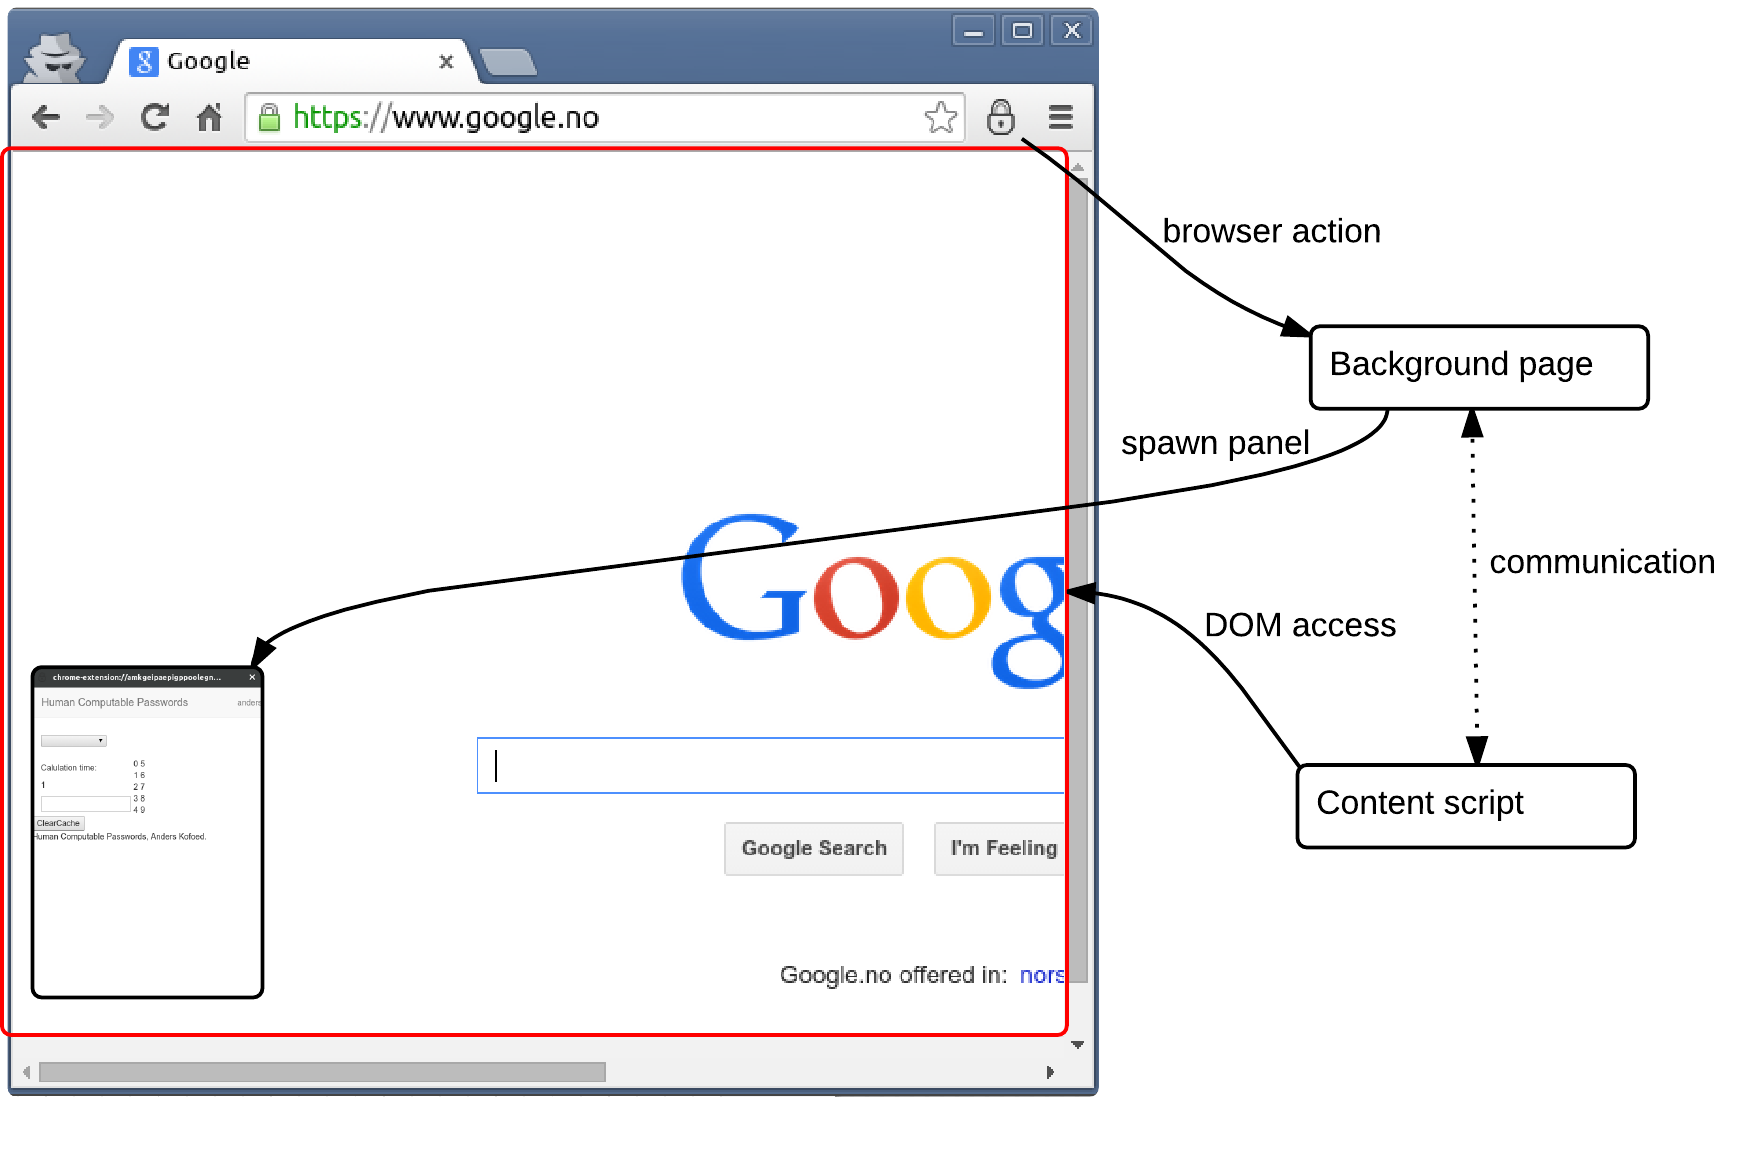
\includegraphics[width=\textwidth]{chrome-extension-ux} }
    \caption{Chrome extensions browser action and content scripts.}
    \label{extension-ux}
\end{figure}

\paragraph{Process isolation} are a set of mechanisms shielding the component from each other and from the web. Usually when javascript is loaded from the web the authority of the script is limited to the origin from where the script is loaded \cite{protecting-browsers}. Since the scripts used by the extensions is loaded from the file system, it does not have a origin in the same sense, and thus needs to be assigned one. This is done by including a public key in the url of the extension, allowing a packaged extensions to sign itself, freeing it from any naming authority or similar. The public key also enables usage of persistent data storage, since the origin of the extension can stay the same throughout updates and patches. This wouldn't be possible otherwise since the chrome local storage API relies on origin.
\par The different components also run in different processes. The content scripts are injected and ran in the same process as the active web page, while the core run in its own process started when the extension is initiated. \todo{paragraph not finished. Cross-origin js and malicious web site operators.}
\par Finally content scripts are ran in a separate javascript environment isolating it from the possibly insecure environment of the web site. The environment of the content scripts are called isolated world, which in practice is a separate set of javascript objects reflecting the ones of the underlying DOM of the web page. This means that the content script can read and edit the DOM of the page it is injected into, but not access variables or javascript functions present in the web page. Both the page and the content scripts sees no other javascript executing in their own isolated world, but they share the same DOM \footnote{Content Scripts, \url{https://developer.chrome.com/extensions/content_scripts} - accessed: 2015-03-05}.

\par \autoref{extension-architecture} illustrates the architecture of chrome extensions with process isolation and isolated worlds.


%
%Instead of running the extensions with the same privileges as the browser, the extensions are ran using only a set of privileges specified before installing \cite{protecting-browsers}. The permissions are specified in a \emph{manifest.json} file, the "permissions" attribute contains the permissions specifying what the extensions will be allowed to do, the manifest file used in this project can be seen in \autoref{manifest}. Note that the only permission used is \emph{storage} which allows access to the chrome storage API. Next, extensions divides permissions between the different components, the content script has access to the content of the active page, and can send messages to the core. As the content script interacts with possibly insecure web pages and thus at risk of being attacked, they are low-privileged. With this division, a compromised content script does not pose a major risk to the core, unless the attacker manages to attack it through the secure messaging channel. The core has access to the extensions APIs, but only those specified in the manifest file as mentioned.
%
%\par In addition chrome extensions are limited  by three levels of isolation. The access to resources are limited to the origin of the extension, to be able to access another origin, typically the current active web page, the cross-origin permission has to be given. In the example manifest this permission is used to allow execution of the file \emph{content\_script} on all urls. In other cases this would be more restrictive, only allowing access to the least amount of origins. The second level of isolation isolates the processes of the content script and the extensions core, with each running in an isolated process. Finally the content script run in a separate javascript environment, an \emph{isolated world}, shielding it from the untrusted content of the active web page. This is meant to protect the extension from web attacks using malicious javascript. The architecture is illustrated in \autoref{extension-architecture} 
%




\begin{figure}[h]
   \fbox{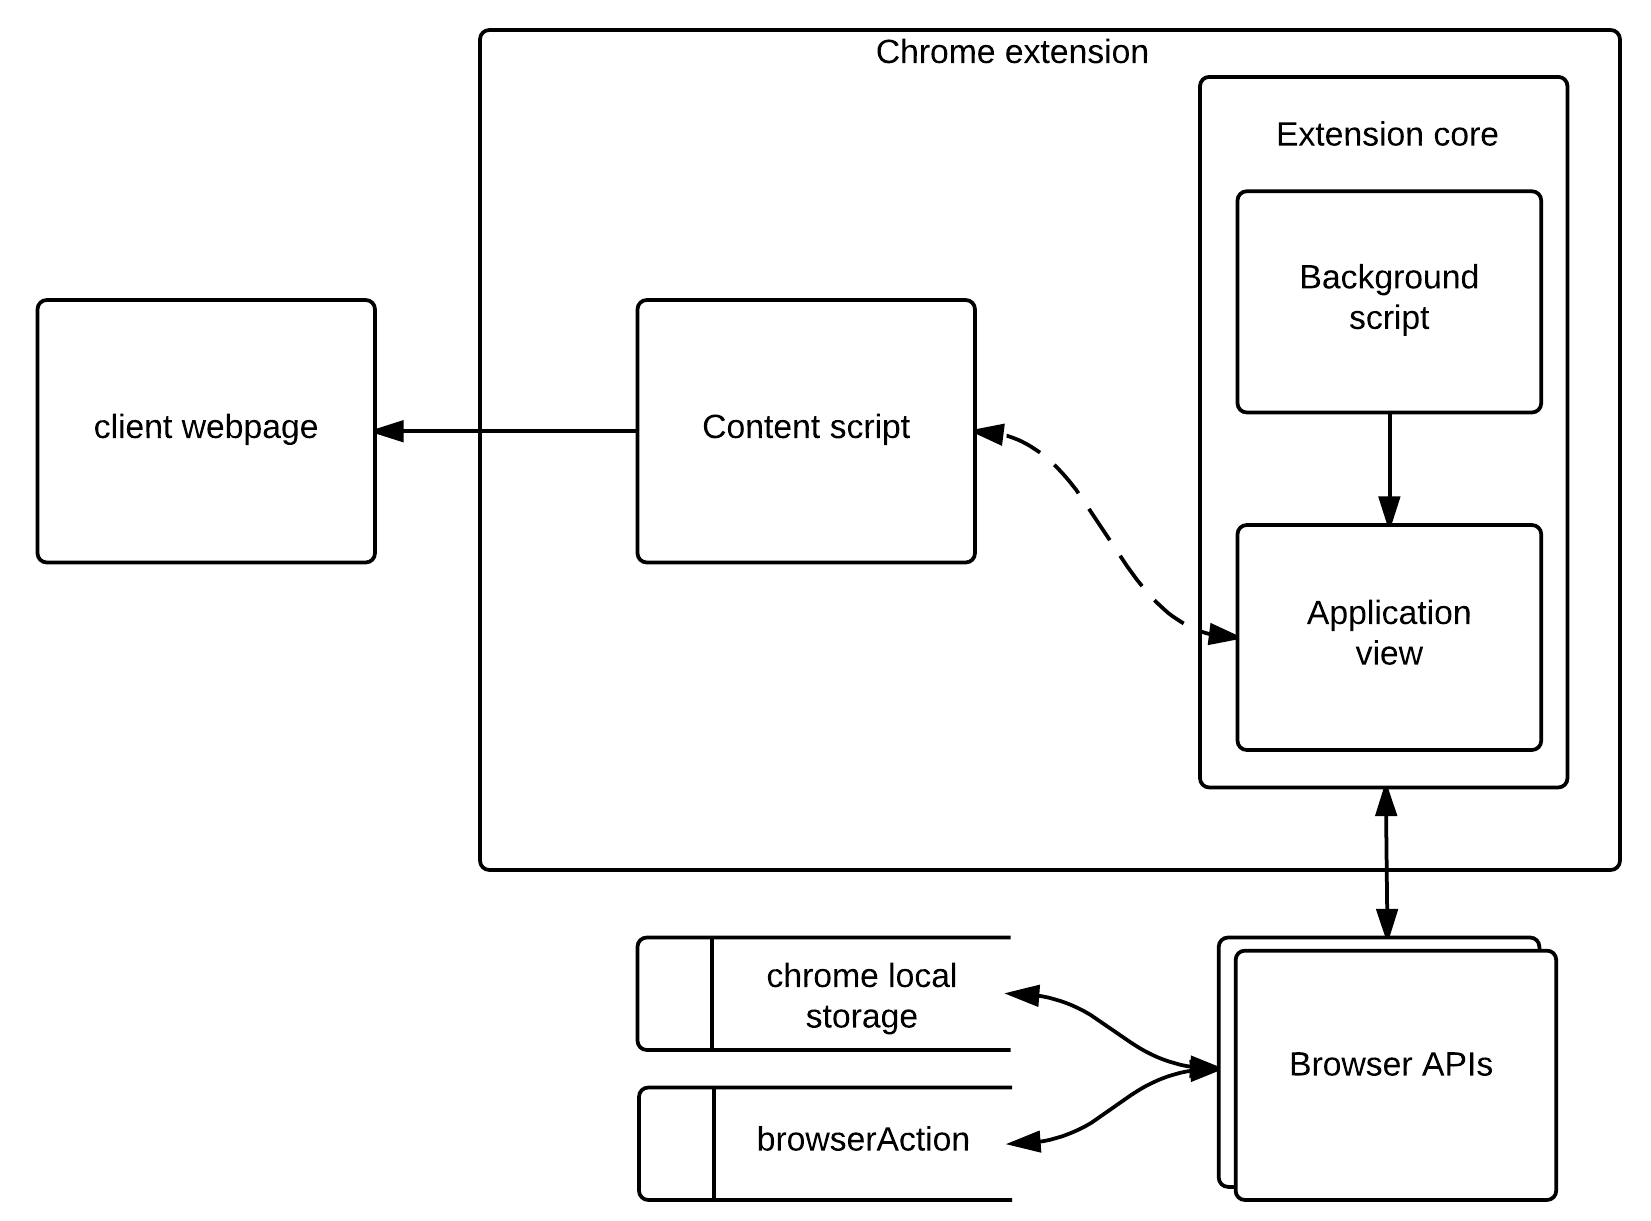
\includegraphics[width=\textwidth]{chrome-extension-architecture} }
    \caption{Chrome extension architecture.}
    \label{extension-architecture}
\end{figure}



